% !Mode:: "TeX:UTF-8"
% !TEX root = ../main.tex
\chapter{网格无关性分析和结果验证}\label{chap: validation}

\section{网格划分}\label{sec: grid}

\subsection{网格生成}

要计算的流动区域如图~\ref{fig: grid}所示。圆柱在二维情形下退化为一圆面,将圆柱的直径设为 1,为了尽可能多地展现出流动情况,将正方形的边长设为 60 倍的圆柱直径,并使圆柱的截面位于正方形的中心位置。整个计算区域以圆为界,分为圆柱内部和圆柱外部两部分,圆柱内部为多孔介质区域,圆柱外部为纯流体区域,圆柱表面为多孔介质区域和纯流体区域的边界。由于采用结构化网格,每个网格均为四边形,为了使圆能被较好地划分,令圆内的网格更加规则,同时使圆柱表面内外的网格尽量光滑衔接,网格尺寸连续变化,于是在圆内再划分出一个正方形,将正方形的边长设置为圆柱直径的一半。这样,整个计算区域就被分成了三个子区域,如图~\ref{fig: grid}所示。

\begin{figure}
	\centering
	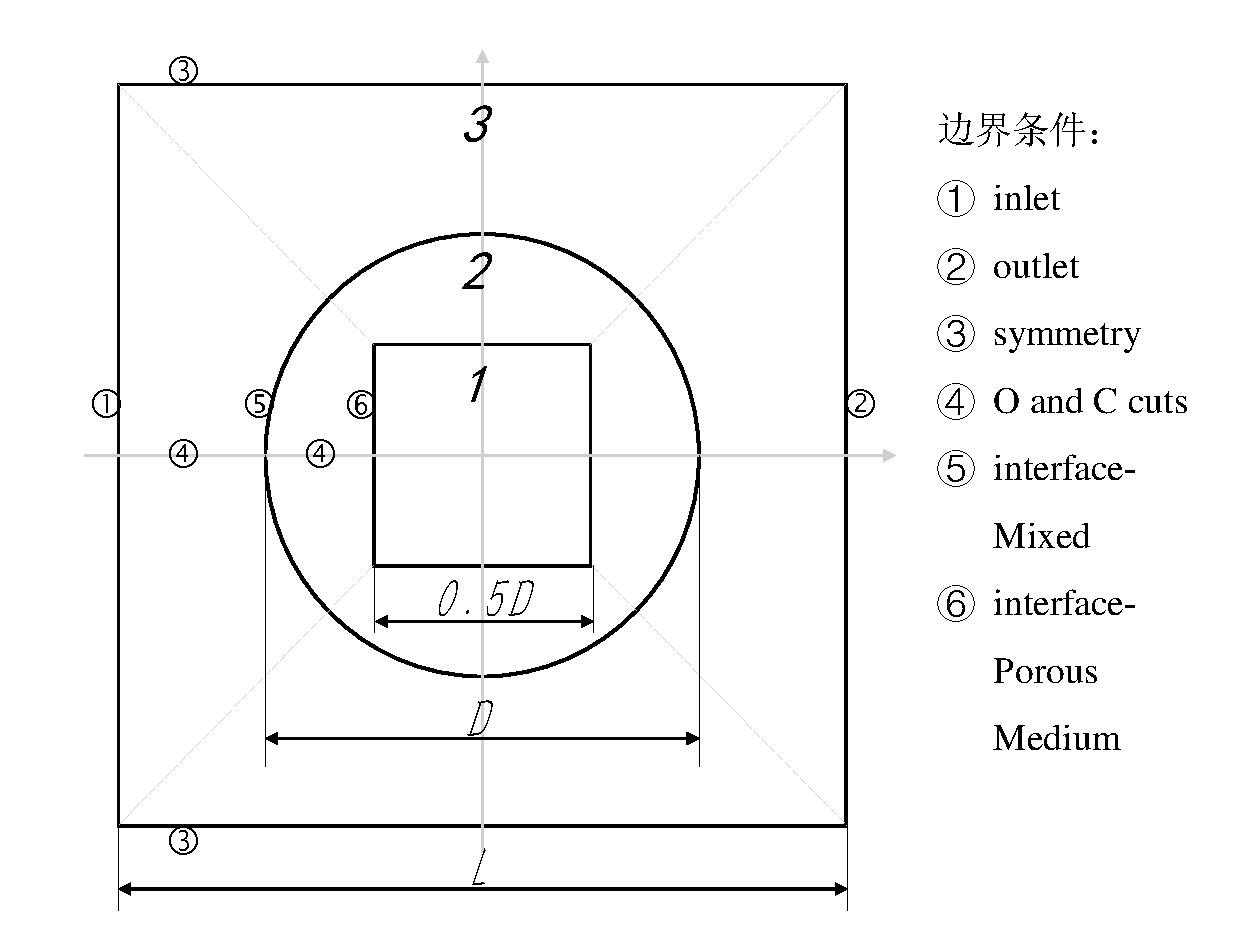
\includegraphics[scale=.7]{figs/grid}
	\caption{网格划分}\label{fig: grid}
\end{figure}

\begin{figure}
	\centering
	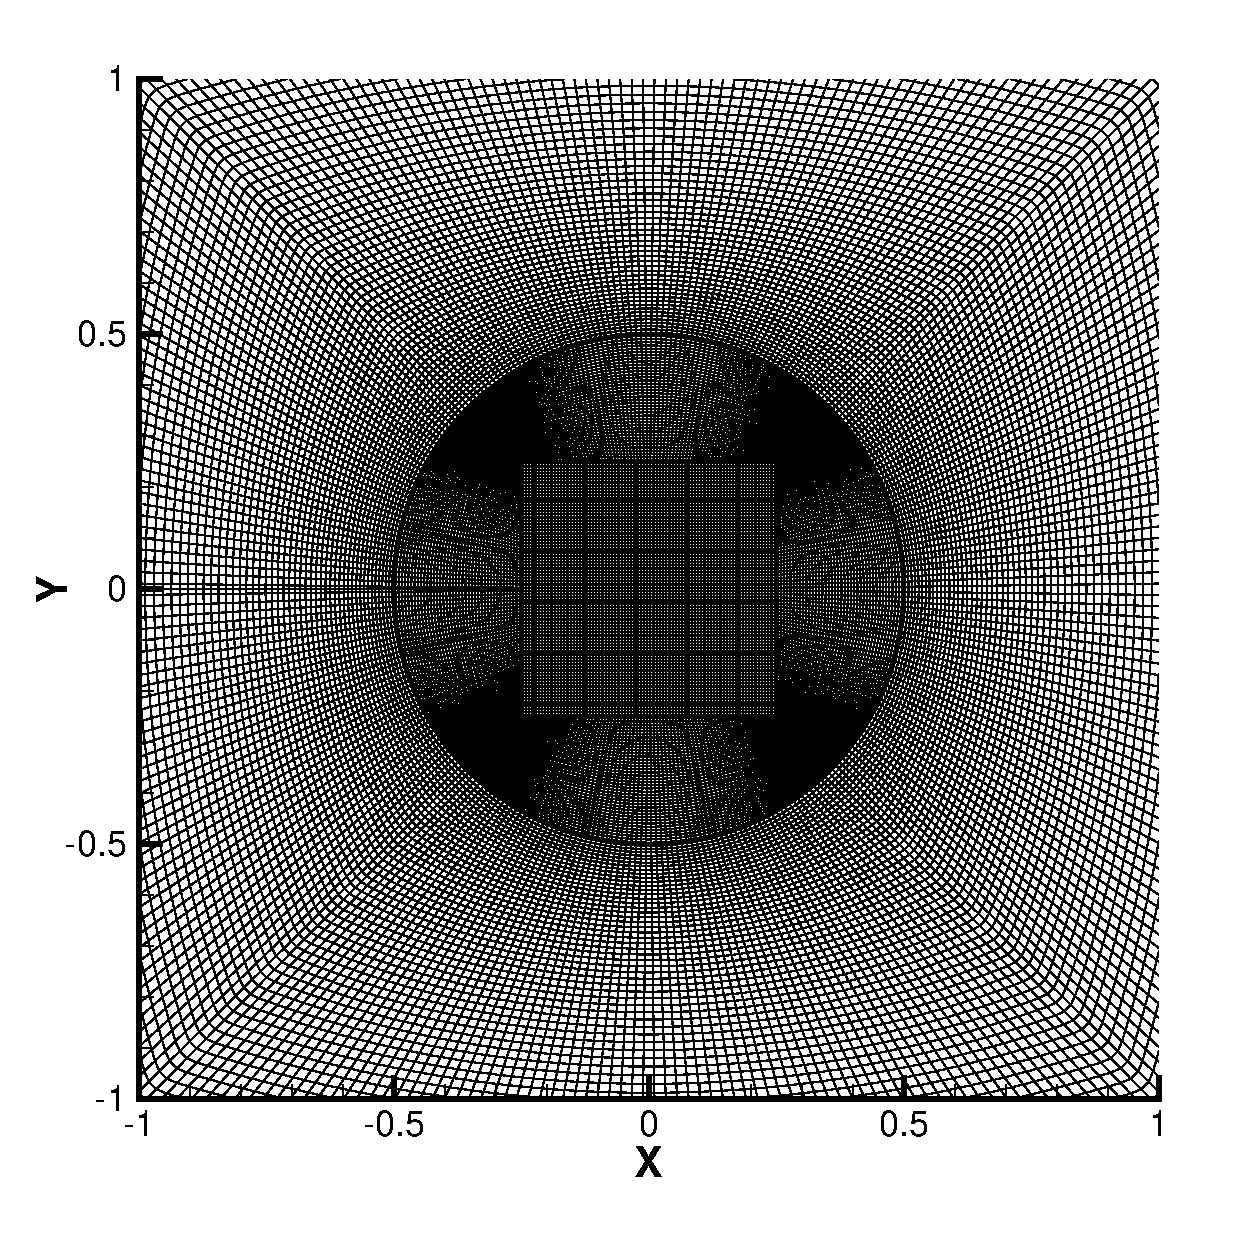
\includegraphics[scale=.7]{figs/grid2}
	\caption{网格划分}\label{fig: grid2}
\end{figure}

在划分网格时,流动区域被分割为连续的小四边形,经纬两个方向的直线织成了整个平面区域。对于第一个子区域(圆内的正方形),只需要将四条边等分,再连接对应点即可。第二个子区域和第三个子区域为 O 型网格。第二个区域的内边界为正方形,外边界为圆,内外表面都被均匀划分,且取相同数量的节点,连接对应的节点形成一条条呈放射状的径向线段,将每一条线段等分,再顺次连接对应的节点,新得到的周向线段与之前的径向线段相交,形成了网状结构,区域被成功划分。第三个区域的内边界为圆,外边界为正方形,两个边界仍然是被均匀划分,连接节点形成径向直线,另一方向的网格划分也和第二个区域类似,不过径向线段不再被等分,而是按照内密外疏的原则依等比数列划分。为了保持圆内外两层网格的大小一致,第三个区域最内侧的网格密度比较大,如果均匀划分,将使网格数过多,而外部网格密度不需要太过细密,所以网格从内到外按照由密到疏的原则进行划分,等比数列是一个较好的选择。另外,为了使圆附近的网格更加细致,第二个区域可以按内疏外密将圆附近的网格适当加密,\ref{subsec: grid-independent}~小节第一组网格的第二个区域就是这样划分的。

\subsection{网格无关性分析}\label{subsec: grid-independent}

解的精度依赖于网格的疏密程度,一般情况下,随着网格数越来越多,网格划分得越来越致密,解的精度也随之提高,但同时计算量也越大,对计算资源的要求也越高。最终应该选择一个合适的网格密度,既使得解能够满足一定的精度要求,同时也可以保持较高的计算效率。为了确保解的精度,需要进行网格无关性验证。选择几种依次递增的网格密度,在同一条件、同一参数下进行数值计算(见表~\ref{tab: parameters}),如果某一网格密度下的解与上一网格密度下的解之差满足了一定的精度要求,就可以认为该网格密度下得到的解已足够精确,从而可以选择该网格密度作为后续模拟的设定值。表~\ref{tab: grid}列出了四种由疏到密的网格尺寸。进行验证的雷诺数和达西数分别为 100 和 0.0001。计算结束后,根据数据得到的平均阻力系数也列在表~\ref{tab: grid}中。表格最后一列的数值表示,与上一行相比,改行平均阻力系数的变化率,即本行的阻力减去上一行的阻力再除以上一行的阻力。

同时设定四个样本点,搜集各个物理量的信息,这四个点的坐标分别是 (0,0),(1,0),(3,0),(1.5,1.5)。通过记录样本点的速度、压强随时间的变化,便于后续分析。

从表~\ref{tab: grid}可以看出,四种情形下计算得到的阻力系数已比较接近,但仍然存在一些差别,网格 2 的阻力系数比网格 1 增大了 0.58\%,网格 3 的阻力系数比网格 2 增大了 0.29\%,网格 4 的阻力系数比网格 3 减小了 0.36\%。因为网格 3 和 2 之间的差别已足够小,达到了 0.3\%,满足了精度要求,所以在后续计算中将采用网格 3 作为数值模拟过程中的网格密度。

\begin{table}[ht]
	\caption{计算参数的设定}\label{tab: parameters}
	\vspace{.5em}\centering\wuhao
	\begin{tabular}{*{8}{c}}
		\toprule[1.5pt]
		$D$ & $L$ & $U_{\infty}$ & $\rho$ & $\varepsilon$ & $\beta_1$ & $\beta_2$ & $\Delta t$\\
		\midrule[1pt]
		1 m & 60 m & 1 m/s & 1 $\mathrm{kg}/\mathrm{m}^3$ & 0.7 & 0 & 0 & 0.001 s\\
		\bottomrule[1.5pt]
	\end{tabular}
\end{table}

\begin{table}[ht]
	\caption{几种不同密度的网格尺寸及相应的阻力系数}\label{tab: grid}
	\vspace{.5em}\centering\wuhao
	\begin{tabular}{cccccc}
		\toprule[1.5pt]
		\multirow{2}[3]{*}{编号} & \multicolumn{3}{c}{网格尺寸} & \multirow{2}[3]{*}{平均阻力系数} & \multirow{2}[3]{*}{阻力系数变化率} \\
		\cmidrule[.67pt](lr){2-4}
		& 区域 1 & 区域 2 & 区域 3 & & \\
		\midrule[1pt]
		1 & 40 $\times$ 40 & 160 $\times$ 25 & 160 $\times$ 140 & 1.2354 & — \\
		2 & 60 $\times$ 60 & 240 $\times$ 30 & 240 $\times$ 170 & 1.2426 & 0.58\% \\
		3 & 80 $\times$ 80 & 320 $\times$ 40 & 320 $\times$ 200 & 1.2462 & 0.29\% \\
		4 & 100 $\times$ 100 & 400 $\times$ 50 & 400 $\times$ 230 & 1.2417 & $-0.36\%$ \\
		\bottomrule[1.5pt]
	\end{tabular}
\end{table}

\section{结果验证}\label{sec: result validation}

确定了网格密度之后,需要验证结果的准确性。已知在多孔圆柱绕流中,达西数决定了多孔介质中流动的程度,当达西数趋于无穷大时,多空区域变成了纯流体区域,当达西数为零时,多空区域则变成了固体区域,内部不再有孔隙,也不再有流体的流动。所以,将达西数设成一个非常小的数值,如果得到的流动状态和已有文献中固体圆柱绕流的流动状态一致,说明结果是准确的。取 $Da=1\times 10^{-5}$ 进行验证。

计算完成后,得到了整个区域的流场特性,即速度、压力以及圆柱受到的阻力和升力系数。根据某一物理量随时间变化的曲线可以得到无量纲频率 Strouhal 数。阻力和升力都随时间做周期性波动,对阻力取出一个周期内的平均值进行比较,对升力则读取波动的振幅进行比较。Strouhal 数、平均阻力、升力振幅的比较见图~\ref{fig: validation-St}、图~\ref{fig: validation-Cd}和图~\ref{fig: validation-Cl}。

以下三幅图展示了多孔介质趋于固体时的流动特性。图~\ref{fig: validation-St}显示了 Strouhal 数随雷诺数的变化,从图中可以看出,在雷诺数从 40 增大到 180 的范围内,当前结果与文献 \inlinecite{Williamson1996} 符合得比较好,$Re=180$ 和 $Re=200$ 两个点和文献不一致,可能是因为这时流动已具有三维特性,所以模拟的结果有一定偏差。

\begin{figure}
	\centering
	\includegraphics[width=0.8\textwidth]{../analysis/validation_St}
	\caption{Strouhal 数的对比}
	\label{fig: validation-St}
\end{figure}

图~\ref{fig: validation-Cd}显示了平均阻力随雷诺数的变化,随着雷诺数的增大,平均阻力逐渐减小,且雷诺数在开始阶段减小很快,之后减小的速度慢慢变小,两条曲线都具有这一趋势,但有一定的差距,与文献 \inlinecite{Rajani2009} 而且文献中的数据在 $Re=60$ 之前下降很快,随后却由一个明显的上升,然后才缓慢下降,这导致曲线在 $Re=60$ 附近不连续,原因尚不明确,可能这是由两段数据组合而成的一个直线。此外,当前研究和文献数据在阻力值上的差距也不明确,只是总体上具有相同的变化趋势。如果在程序中不考虑达西数,而不是将达西数设为一个很小的值,那么得到的结果会更接近文献数据。所以,这一差距可能由达西数的加入而引起。

\begin{figure}[ht]
	\centering
	\includegraphics[width=0.8\textwidth]{../analysis/validation_Cd}
	\caption{平均阻力系数 $C_D$ 的对比}
	\label{fig: validation-Cd}
\end{figure}

图~\ref{fig: validation-Cl}显示了升力振幅随雷诺数的变化,升力波动的振幅均随雷诺数的增大而增大,且二者基本吻合。总体而言,当前结果与文献在一定程度上是一致的,经过验证,结果基本准确。

\begin{figure}[ht]
	\centering
	\includegraphics[width=0.8\textwidth]{../analysis/validation_Cl}
	\caption{升力系数 $C_L$ 的对比}
	\label{fig: validation-Cl}
\end{figure}

\section{本章小结}

本章

\ref{sec: grid} 节定义了该问题的计算区域,将正方形的计算区域划分为三个子域,在每个区域内划分出正交网格,并规定每两块网格之间的边界条件。为了寻找合适的网格分辨率,在取得足够精度的同时又保证一定计算效率,进行了网格无关性验证。通过在相同的参数下设定一系列的网格密度,分别计算,对得到的结果进行分析,发现 $80\times 80$ 的网格具有足够的精度,将作为后续计算的设定。\ref{sec: result validation} 节通过将达西数设为 $1\times 10^{-5}$ 进行计算,并和已有的固体圆柱绕流结果比对,确定了计算的准确性。
